%! TEX root = main.tex

\chapter{2D Continuous Systems}

Many sound-radiating structures in musical instruments are not one-dimensional: drumheads, membranes, thin plates and shells are spatially extended in two directions. Their vibration is described by partial differential equations in two spatial variables and the observed motion results from wave propagation on a surface, reflections at boundaries and the formation of 2D standing-wave patterns (modes). This chapter introduces the fundamental 2D models (membranes and plates), derive their wave equations and obtain the modal shapes and eigenfrequencies for simple geometries.

\section{Wave Equation for a Rectangular Membrane}

Consider a rectangular membrane of dimensions \( L_x \) and \( L_y \), under uniform tension \( T \) (\si{\newton\per\metre}) and with mass density per unit area \( \sigma \) (\si{\kilo\gram\per\metre\squared}). Let \( z(x,y,t) \) denote the transverse displacement.

\subsection{Derivation of the Membrane Wave Equation}

\begin{figure}[!htb]
    \centering
    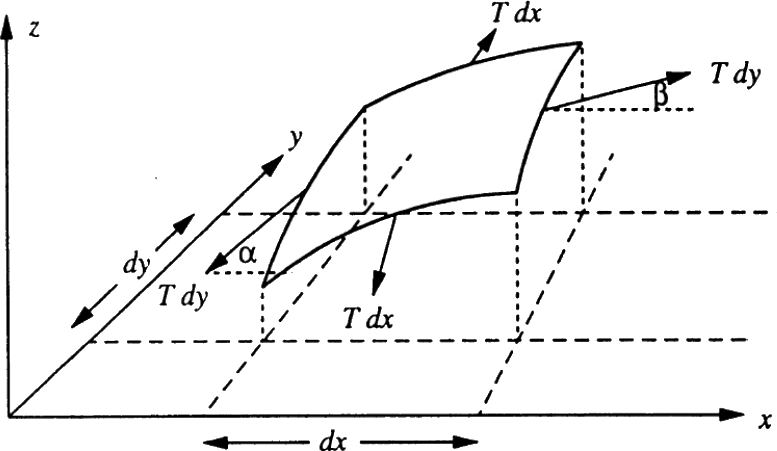
\includegraphics[width=0.75\linewidth]{00_Images/03_chapter/01.png}
    \caption{Forces on an infinitesimal membrane element under uniform tension}
    \label{fig:membrane_element}
\end{figure}

Take an infinitesimal element of membrane with sides \( dx \) and \( dy \). The tension acting on the edge of length \( dx \) is \( Tdx \) (and similarly on the edge \( dy \)). For small slopes, the vertical components of these tensions provide the restoring force. Summing the net vertical force contributions in the \( x \) and \( y \) directions and applying Newton's second law to the element of mass \( \sigma dxdy \) yields the membrane equation of motion:
\[
\frac{\partial^{2}z}{\partial t^{2}}
 = 
\frac{T}{\sigma}
\left(
\frac{\partial^{2}z}{\partial x^{2}}
+
\frac{\partial^{2}z}{\partial y^{2}}
\right)
 = 
c^{2}\nabla^{2}z,
\qquad
c = \sqrt{\frac{T}{\sigma}}
\]
Here \( c \) is the wave speed on the membrane and \( \nabla^{2} \) is the 2D Laplacian in Cartesian coordinates.

\subsection{Separation of Variables and Harmonic Solutions}

For a rectangular domain it is natural to work in Cartesian coordinates and seek separable solutions of the form
\[
z(x,y,t) = X(x)Y(y)\Phi(t)
\]
Substitution gives
\[
\frac{1}{\Phi}\frac{d^{2}\Phi}{dt^{2}}
 = 
c^{2}\left(
\frac{1}{X}\frac{d^{2}X}{dx^{2}}
+
\frac{1}{Y}\frac{d^{2}Y}{dy^{2}}
\right)
\]
Since the left-hand side depends only on \( t \) and the right-hand side depends only on \( x,y \), both must be equal to the same constant. Choosing the constant as \( -\omega^{2} \) yields
\[
\frac{d^{2}\Phi}{dt^{2}}+\omega^{2}\Phi = 0
\quad\Rightarrow\quad
\Phi(t) = E\sin\omega t+F\cos\omega t
\]
and, for the spatial part,
\[
\frac{1}{X}\frac{d^{2}X}{dx^{2}}+\frac{\omega^{2}}{c^{2}}
 = 
-\frac{1}{Y}\frac{d^{2}Y}{dy^{2}}
\]
For this to hold at every point, it sets
\[
\frac{1}{X}\frac{d^{2}X}{dx^{2}} = -h^{2},
\qquad
\frac{1}{Y}\frac{d^{2}Y}{dy^{2}} = -r^{2},
\qquad
h^{2}+r^{2} = \frac{\omega^{2}}{c^{2}}
\]
so that
\[
X(x) = A\sin(hx)+B\cos(hx),
\qquad
Y(y) = C\sin(ry)+D\cos(ry)
\]
The parameters \( h \) and \( r \) determine the spatial periodicity along \( x \) and \( y \), respectively. 

\subsection{Fixed-Edge Boundary Conditions and Natural Frequencies}

For a membrane clamped along its boundary, the displacement vanishes at the edges:
\[
z = 0 \quad \text{at} \quad x = 0,\ x = L_x,\ y = 0,\ y = L_y
\]
The conditions at \( x = 0 \) and \( y = 0 \) imply \( B = 0 \) and \( D = 0 \). Imposing \( z(L_x,y,t) = 0 \) requires
\[
\sin(hL_x) = 0 \quad\Rightarrow\quad h = \frac{m\pi}{L_x},
\qquad m = 1,2,3,\dots
\]
and imposing \( z(x,L_y,t) = 0 \) requires
\[
\sin(rL_y) = 0 \quad\Rightarrow\quad r = \frac{n\pi}{L_y},
\qquad n = 1,2,3,\dots
\]
Therefore the \( (m,n) \) -th mode shape is
\[
z_{mn}(x,y,t) = A\sin\left(\frac{m\pi}{L_x}x\right)\sin\left(\frac{n\pi}{L_y}y\right)
\left(E\sin\omega_{mn}t+F\cos\omega_{mn}t\right)
\]
with
\[
\omega_{mn} = c\sqrt{h^{2}+r^{2}}
 = 
c\pi\sqrt{\left(\frac{m}{L_x}\right)^{2}+\left(\frac{n}{L_y}\right)^{2}}
\]
and the natural frequencies
\[
f_{mn} = \frac{\omega_{mn}}{2\pi}
 = 
\frac{1}{2}\sqrt{\frac{T}{\sigma}}
\sqrt{\left(\frac{m}{L_x}\right)^{2}+\left(\frac{n}{L_y}\right)^{2}}
\]
As usual, \( m = 0 \) or \( n = 0 \) (and in particular \( m = n = 0 \)) corresponds to the trivial solution \( z = 0 \).

\paragraph{Square membranes and modal degeneracy} If \( L_x = L_y \), then \( f_{mn} = f_{nm} \): distinct mode shapes can share the same eigenfrequency. In that case, any linear combination
\[
z(x,y,t) = \left(az_{mn}+bz_{nm}\right)\cos\omega t,
\qquad a^{2}+b^{2} = 1
\]
is also a valid vibration pattern at the same frequency and the observed nodal lines depend on the combination coefficients.

\begin{figure}[!htb]
    \centering
    \subfloat[Degenerate modes in a square membrane]{%
        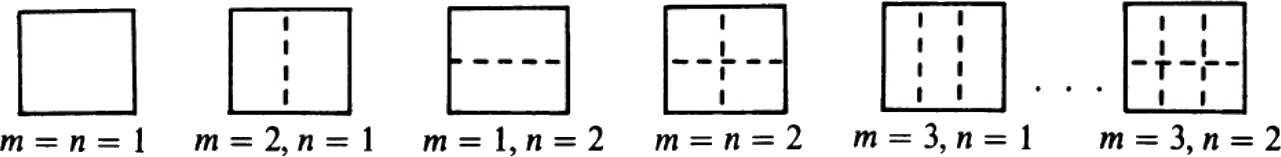
\includegraphics[width=0.9\linewidth]{00_Images/03_chapter/02.png}%
    }\\
    \subfloat[Linear combinations and resulting nodal patterns]{%
        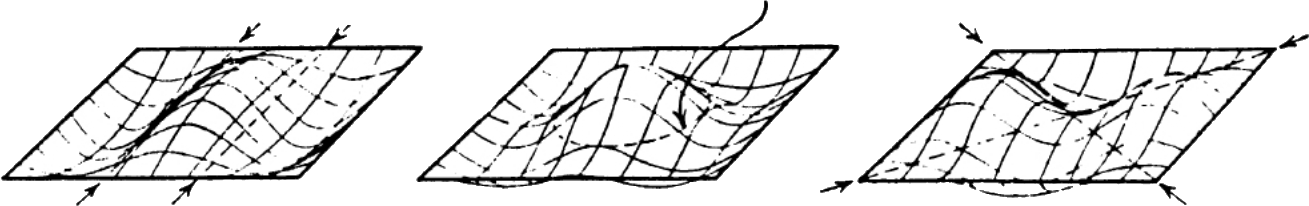
\includegraphics[width=0.9\linewidth]{00_Images/03_chapter/03.png}%
    }
    \caption{Modal degeneracy in a square membrane}
    \label{fig:square_membrane_degeneracy}
\end{figure}

\section{Circular Membranes}

For a circular membrane the boundary condition imposes that the transverse displacement vanishes on the circular edge. It places the origin at the center of the membrane, uses polar coordinates \( (r,\varphi) \) and denotes by \( a \) the membrane radius.

\subsection{Wave Equation in Polar Coordinates}

For a membrane under uniform tension \( T \) (\si{\newton\per\metre}) and surface mass density \( \sigma \) (\si{\kilo\gram\per\metre\squared}), the equation of motion becomes
\[
\frac{\partial^{2}z}{\partial t^{2}}
 = 
c^{2}\left(
\frac{\partial^{2}z}{\partial r^{2}}
+\frac{1}{r}\frac{\partial z}{\partial r}
+\frac{1}{r^{2}}\frac{\partial^{2}z}{\partial \varphi^{2}}
\right),
\qquad
c = \sqrt{\frac{T}{\sigma}}
\]
The clamped-edge condition is
\[
z(a,\varphi,t) = 0 \quad \text{for all } \varphi,t
\]

\subsection{Separation of Variables and Bessel Functions}

\begin{figure}[!htb]
    \centering
    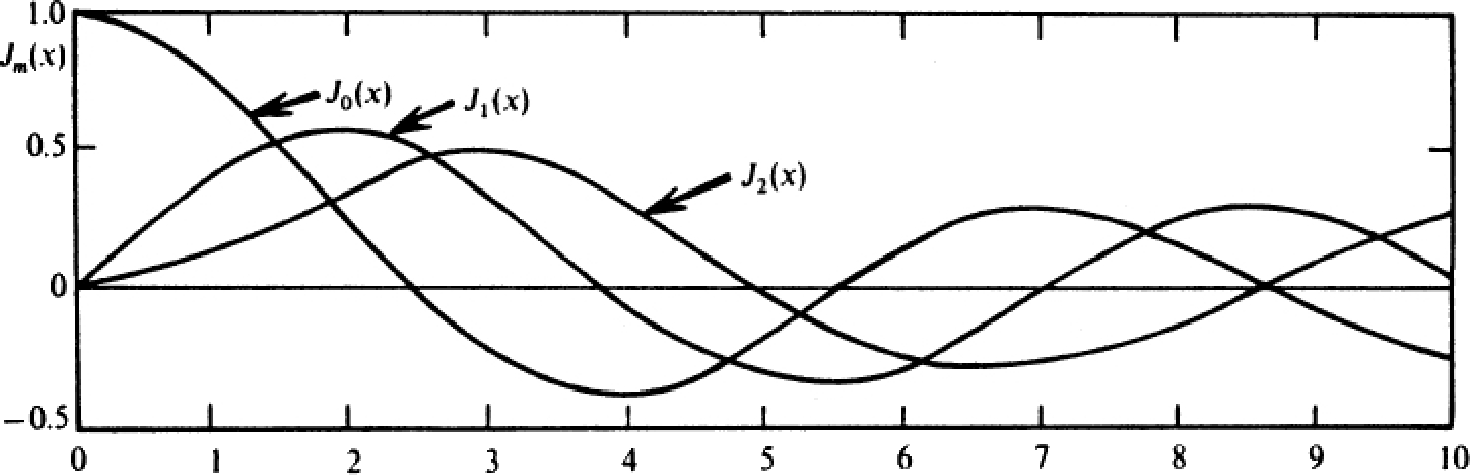
\includegraphics[width=0.8\linewidth]{00_Images/03_chapter/04.png}
    \caption{Bessel functions (first kind) and their zeros}
    \label{fig:bessel_zeros}
\end{figure}

Assume a harmonic separable solution
\[
z_e(r,\varphi,t) = R(r)\Phi(\varphi)e^{j\omega t}
\]
Substitution yields two ordinary differential equations. The angular part is
\[
\frac{d^{2}\Phi}{d\varphi^{2}}+m^{2}\Phi = 0
\qquad\Rightarrow\qquad
\Phi(\varphi) = A e^{\pm jm\varphi}
\]
where \( m\in\mathbb{Z} \) is the azimuthal order. The radial part becomes
\[
\frac{d^{2}R}{dr^{2}}+\frac{1}{r}\frac{dR}{dr}
+\left(\frac{\omega^{2}}{c^{2}}-\frac{m^{2}}{r^{2}}\right)R = 0
\]
This is Bessel's equation. The physically acceptable solution at \( r = 0 \) is the Bessel function of the first kind,
\[
R(r) = J_m(kr),
\qquad
k = \frac{\omega}{c}
\]

\subsection{Boundary Condition, Eigenvalues and Natural Frequencies}

The clamped boundary condition \( z(a,\varphi,t) = 0 \) implies
\[
J_m(ka) = 0
\]
Let \( Z_{mn} \) denote the \( n \) -th positive zero of \( J_m(\cdot) \). Then the admissible wavenumbers are
\[
k_{mn} = \frac{Z_{mn}}{a}
\]
and the natural (angular) frequencies are
\[
\omega_{mn} = ck_{mn} = c\frac{Z_{mn}}{a},
\qquad
f_{mn} = \frac{\omega_{mn}}{2\pi}
 = 
\frac{Z_{mn}}{2\pi a}\sqrt{\frac{T}{\sigma}}
\]
As an example, for the fundamental axisymmetric mode \( (m,n) = (0,1) \) one has \( Z_{01} \simeq 2.405 \), hence
\[
f_{01} = 
\frac{2.405}{2\pi a}\sqrt{\frac{T}{\sigma}}
\]

\subsection{Mode Shapes and Nodal Patterns}

\begin{figure}[!htb]
    \centering
    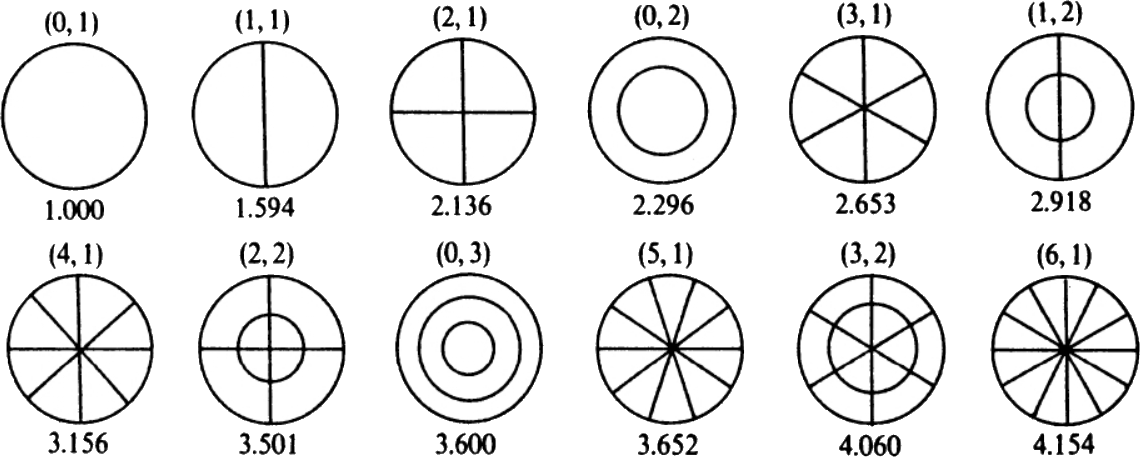
\includegraphics[width=0.9\linewidth]{00_Images/03_chapter/05.png}
    \caption{Normal modes of a circular membrane (nodal diameters and circles)}
    \label{fig:circular_membrane_modes}
\end{figure}

The (complex) modal shape can be written as
\[
z_{emn}(r,\varphi) = \Phi(\varphi)R(r) = A e^{\pm jm\varphi}J_m(k_{mn}r)
\]
and the overall (complex) displacement is a modal superposition
\[
z_e(r,\varphi,t) = \sum_{m}\sum_{n} c_{mn}z_{emn}(r,\varphi)e^{j\omega_{mn}t},
\qquad
z(r,\varphi,t) = \Re\{z_e(r,\varphi,t)\}
\]
where the coefficients \( c_{mn} \) depend on the excitation. Geometrically, the \( (m,n) \) -th mode has:

\begin{itemize}
    \item \( m \) nodal diameters (lines through the center);
    \item \( n \) nodal circles (concentric rings), counting the boundary as the outer zero.
\end{itemize}

In particular, \( (0,1) \) entails an in-phase displacement of the whole membrane, while \( (1,1) \) is an antisymmetric motion of the two halves. 

\paragraph{Remark on air loading} When the membrane is in contact with air, modal frequencies are generally lowered. In a kettledrum, where the air is confined, axisymmetric modes such as \( (0,1) \) are raised, while the remaining modes are lowered. 

\section{Elastic Materials and Mechanical Parameters}

Now, it is useful to summarize the constitutive parameters that control wave propagation in solids. In continuum mechanics, external loads generate a stress field, which in turn produces a strain field according to material-dependent constitutive equations. For linear elastic media, these relations are linear and can be expressed compactly in tensor or matrix form. 

\subsection{Stress, Strain and Generalized Hooke's Law}

Consider a deformable solid (e.g. a small cube). The stress tensor \( \sigma_{ij} \) represents the force per unit area acting on the face orthogonal to axis \( i \), directed along axis \( j \). Similarly, the strain tensor \( \varepsilon_{kl} \) quantifies the deformation. In matrix form,
\[
\symbf{\sigma} = 
\begin{bmatrix}
\sigma_{xx} & \sigma_{xy} & \sigma_{xz}\\
\sigma_{yx} & \sigma_{yy} & \sigma_{yz}\\
\sigma_{zx} & \sigma_{zy} & \sigma_{zz}
\end{bmatrix},
\qquad
\symbf{\varepsilon} = 
\begin{bmatrix}
\varepsilon_{xx} & \varepsilon_{xy} & \varepsilon_{xz}\\
\varepsilon_{yx} & \varepsilon_{yy} & \varepsilon_{yz}\\
\varepsilon_{zx} & \varepsilon_{zy} & \varepsilon_{zz}
\end{bmatrix}
\]
In general, a single stress component \( \sigma_{ij} \) can generate several strain components \( \varepsilon_{kl} \). The most general linear elastic constitutive relation is the generalized Hooke's law
\[
\sigma_{ij} = A_{ijkl}\varepsilon_{kl}
\]
where \( A_{ijkl} \) is the elasticity tensor (fourth-rank). It has \( 3^4 = 81 \) components, reduced by symmetry considerations (stress and strain tensors are symmetric) and by energy arguments down to 21 independent constants in the fully anisotropic case. 

\subsection{Uniaxial Traction: Young's Modulus and Yield Strength}

\begin{figure}[!htb]
    \centering
    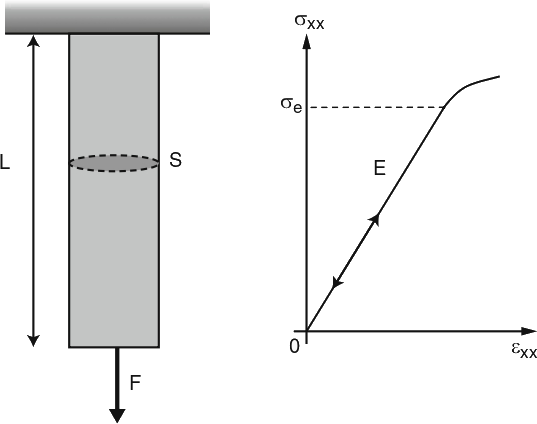
\includegraphics[width=0.6\linewidth]{00_Images/03_chapter/06.png}
    \caption{Uniaxial traction and a typical stress-strain curve}
    \label{fig:uniaxial_traction}
\end{figure}

A basic experiment to characterize stiffness is uniaxial traction of a slender specimen (length \( L_0 \) much larger than its lateral size). If a tensile force \( F \) is applied along \( x \), the axial stress and strain are approximated by
\[
\sigma_{xx} \simeq \frac{F}{S},
\qquad
\varepsilon_{xx} \simeq \frac{L-L_0}{L_0}
\]
In the linear reversible regime (below the yield strength \( \sigma_e \)), stress and strain are proportional,
\[
\sigma_{xx} = E\varepsilon_{xx}
\]
where \( E \) is Young's modulus. Beyond \( \sigma_e \), the stress-strain curve is no longer linear and at higher stress the specimen ultimately fails (ultimate tensile strength). Typical values for \( E \), \( \sigma_e \) and ultimate strength vary greatly across materials (metals, polymers, glass, etc.). 

\subsection{Poisson's Ratio and the Poisson Effect}

\begin{figure}[!htb]
    \centering
    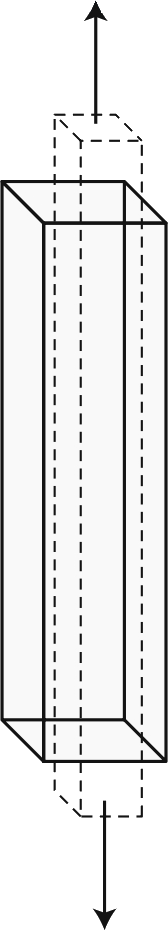
\includegraphics[height=0.3\textheight]{00_Images/03_chapter/07.png}
    \caption{Poisson effect under uniaxial loading}
    \label{fig:poisson_effect}
\end{figure}

Under uniaxial traction along \( x \), real solids  contract laterally. In the simplest isotropic linear model, 
\[
\varepsilon_{yy} = -\nu\frac{\sigma_{xx}}{E},
\qquad
\varepsilon_{zz} = -\nu\frac{\sigma_{xx}}{E}
\]
where \( \nu \) is Poisson's ratio. Thus \( \nu \) measures the lateral compression under axial extension (Poisson effect). For most standard materials \( 0<\nu<1/2 \), but special auxetic materials exhibit an effective \( \nu<0 \), i.e. they expand laterally when stretched due to their microstructure. 

\subsection{Shear Modulus}

\begin{figure}[!htb]
    \centering
    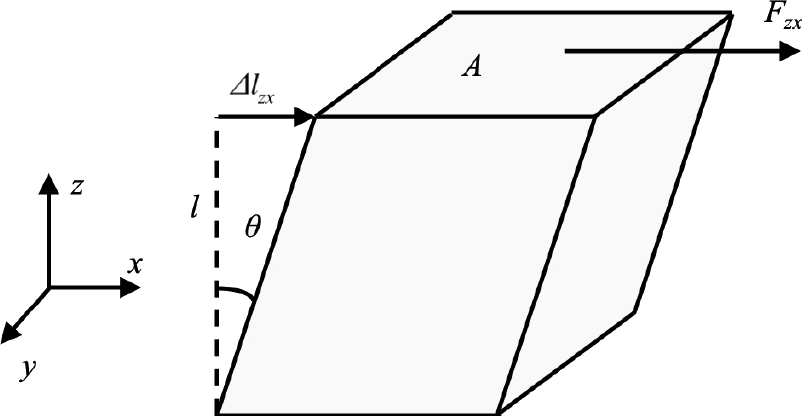
\includegraphics[width=0.65\linewidth]{00_Images/03_chapter/08.png}
    \caption{Shear deformation defining the shear modulus \(G\)}
    \label{fig:shear_modulus}
\end{figure}

A second independent elastic parameter is the shear (torsional) modulus \( G \), defined as the ratio between shear stress and shear strain. For the shear component \( (z,x) \), 
\[
G = \frac{\sigma_{zx}}{\gamma_{zx}}
 = 
\frac{F_{zx}/A}{\Delta l_{zx}/l}
 = 
\frac{F_{zx}l}{A\Delta l_{zx}}
\]
where \( A \) is the sheared area, \( l \) the specimen height and \( \gamma_{zx}\simeq\tan\theta \simeq \theta \) is the (small) shear strain. Values of \( G \) also span orders of magnitude across materials. 

\subsection{Voigt Notation and Matrix Constitutive Equations}

Because \( \sigma \) and \( \varepsilon \) are symmetric, it is convenient to collect their independent components into 6-vectors (Voigt notation):
\[
\vv{\sigma}_V = 
\begin{bmatrix}
\sigma_{xx}&\sigma_{yy}&\sigma_{zz}&\sigma_{zx}&\sigma_{yz}&\sigma_{xy}
\end{bmatrix}^{T},
\qquad
\vv{\varepsilon}_V = 
\begin{bmatrix}
\varepsilon_{xx}&\varepsilon_{yy}&\varepsilon_{zz}&\varepsilon_{zx}&\varepsilon_{yz}&\varepsilon_{xy}
\end{bmatrix}^{T}
\]
Then the constitutive law becomes a \( 6 \times 6 \) matrix relation,
\[
\vv{\sigma}_V = \symbf{A}_V\vv{\varepsilon}_V
\]
This form is particularly useful in plate and shell models, where bending stiffness and wave propagation constants can be expressed directly in terms of elastic matrix entries.

\subsection{Isotropic Materials: the Lamé Parameters}

In an isotropic material all directions are equivalent and linear elasticity is fully characterized by two constants (Lamé parameters \( \lambda \) and \( \mu \)). In Voigt notation the stiffness matrix takes the standard form
\[
\begin{bmatrix}
\sigma_{xx}\\\sigma_{yy}\\\sigma_{zz}\\\sigma_{zx}\\\sigma_{yz}\\\sigma_{xy}
\end{bmatrix}
 = 
\begin{bmatrix}
\lambda+2\mu & \lambda      & \lambda      & 0   & 0   & 0\\
\lambda      & \lambda+2\mu & \lambda      & 0   & 0   & 0\\
\lambda      & \lambda      & \lambda+2\mu & 0   & 0   & 0\\
0            & 0            & 0            & 2\mu& 0   & 0\\
0            & 0            & 0            & 0   & 2\mu& 0\\
0            & 0            & 0            & 0   & 0   & 2\mu
\end{bmatrix}
\begin{bmatrix}
\varepsilon_{xx}\\\varepsilon_{yy}\\\varepsilon_{zz}\\\varepsilon_{zx}\\\varepsilon_{yz}\\\varepsilon_{xy}
\end{bmatrix}
\]
The Lamé parameters can be expressed in terms of Young's modulus \( E \) and Poisson's ratio \( \nu \) as:
\[
\lambda = \frac{E\nu}{(1+\nu)(1-2\nu)},
\qquad
\mu = \frac{E}{2(1+\nu)}
\]
In particular, \( \mu \) coincides with the shear modulus \( G \) for isotropic media.

\subsection{Orthotropic Materials: Wood and Directional Elasticity}

\begin{figure}[!htb]
    \centering
    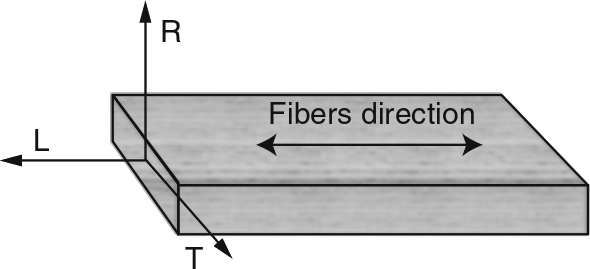
\includegraphics[width=0.78\linewidth]{00_Images/03_chapter/09.png}
    \caption{Orthotropic axes in wood: longitudinal (L), radial (R), tangential (T)}
    \label{fig:wood_axes}
\end{figure}

Many musical materials are anisotropic. Wood is often modeled as orthotropic, meaning that its elastic properties differ along three orthogonal material directions: longitudinal \( L \) (along the fibers), radial \( R \) (along growth-ring radii) and tangential \( T \) (tangent to growth rings). In this case, it is convenient to write the compliance form (strain as a function of stress). For axes aligned with \( x = L \), \( y = R \), \( z = T \), the Voigt relation becomes:
\[
\begin{bmatrix}
\varepsilon_{xx}\\\varepsilon_{yy}\\\varepsilon_{zz}\\\varepsilon_{zx}\\\varepsilon_{yz}\\\varepsilon_{xy}
\end{bmatrix}
 = 
\begin{bmatrix}
\frac{1}{E_L} & -\frac{\nu_{RL}}{E_R} & -\frac{\nu_{TL}}{E_T} & 0 & 0 & 0\\
-\frac{\nu_{LR}}{E_L} & \frac{1}{E_R} & -\frac{\nu_{TR}}{E_T} & 0 & 0 & 0\\
-\frac{\nu_{LT}}{E_L} & -\frac{\nu_{RT}}{E_R} & \frac{1}{E_T} & 0 & 0 & 0\\
0 & 0 & 0 & \frac{1}{2G_{LT}} & 0 & 0\\
0 & 0 & 0 & 0 & \frac{1}{2G_{TR}} & 0\\
0 & 0 & 0 & 0 & 0 & \frac{1}{2G_{RL}}
\end{bmatrix}
\begin{bmatrix}
\sigma_{xx} \\
\sigma_{yy} \\
\sigma_{zz} \\
\sigma_{zx} \\
\sigma_{yz} \\
\sigma_{xy}
\end{bmatrix}
\]
The orthotropic elastic behavior is described by nine independent coefficients: 

\begin{itemize}
    \item three Young's moduli \( E_L, E_R, E_T \),
    \item three Poisson ratios (e.g. \( \nu_{LR}, \nu_{RT}, \nu_{TL} \)),
    \item three shear moduli \( G_{LT}, G_{TR}, G_{RL} \).
\end{itemize}

The remaining Poisson ratios are determined by symmetry constraints (\( \nu_{LR}/E_L = \nu_{RL}/E_R \) and similarly for the other pairs). For spruce soundboards, a typical feature is the strong anisotropy \( E_L/E_T \) (often of order \( 10 \) to \( 20 \)), which is one of the key reasons why the orientation of the grain matters in instrument making. 

\section{Waves in Thin Plates}

The previous section introduced the elastic constants (\( E,\nu,G \)) and the density \( \rho \), which fully determine (together with thickness \( h \)) the propagation of mechanical waves in thin plates. Unlike membranes, plates possess bending stiffness, so waves can propagate even in the absence of any applied in-plane tension. In thin plates three main families of waves are commonly distinguished: quasi-longitudinal waves, torsional (in-plane shear) waves and bending (flexural) waves.

\begin{figure}[!htb]
    \centering
    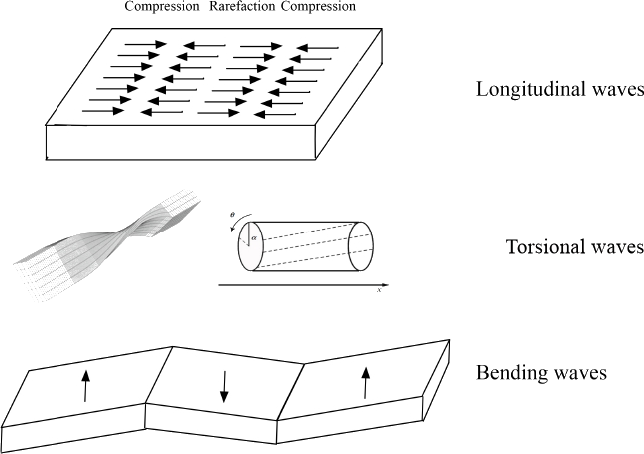
\includegraphics[width=0.6\linewidth]{00_Images/03_chapter/10.png}
    \caption{Wave types in thin plates: quasi-longitudinal, torsional, and bending}
    \label{fig:plate_wave_types}
\end{figure}

\subsection{Quasi-Longitudinal Waves}

\begin{figure}[!htb]
    \centering
    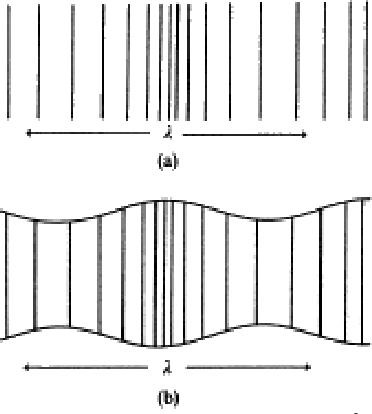
\includegraphics[width=0.5\linewidth]{00_Images/03_chapter/11.png}
    \caption{Quasi-longitudinal deformation in a thin plate}
    \label{fig:quasi_longitudinal_plate}
\end{figure}

Longitudinal waves in plates do not propagate at the same speed as longitudinal waves in bars made of the same material. When a longitudinal wave propagates in a thin plate, it induces a slight expansion/compression in the direction orthogonal to the wavefront through the Poisson effect; this modifies the local stiffness and changes the wave speed. For this reason they are referred to as quasi-longitudinal waves. Purely longitudinal waves occur only in solids whose dimensions are all much larger than the wavelength. The propagation velocity of quasi-longitudinal waves in a plate is
\[
c_L = \sqrt{\frac{E}{\rho(1-\nu^{2})}}
\]
where \( E \) is Young's modulus, \( \rho \) is the material density and \( \nu \) is Poisson's ratio. For comparison, a purely longitudinal wave (3D bulk) would propagate at
\[
c_L' = \sqrt{\frac{E(1-\nu)}{\rho(1+\nu)(1-2\nu)}}
\]
while the classical 1D bar result is
\[
c_{L,\mathrm{bar}} = \sqrt{\frac{E}{\rho}}
\]
These expressions make explicit that the plate velocity differs from the bar velocity because \( \nu\neq 0 \) couples axial and lateral strains. 

\subsection{Torsional (In-Plane Shear) Waves}

Torsional waves in a thin plate propagate at the same speed as torsional waves in a rod, namely
\[
c_T = \sqrt{\frac{G}{\rho}}
\]
where \( G \) is the shear modulus. Since typically \( G<E \), torsional waves propagate slower than longitudinal (or quasi-longitudinal) waves. Torsional and quasi-longitudinal waves involve particle motion that is largely tangential to the plate surface; consequently, they are comparatively inefficient for airborne sound radiation. In musical applications they may still be relevant because their modal frequencies are generally not in harmonic correspondence with the main flexural components and can therefore produce perceptually annoying or unexpected features if strongly excited.

\subsection{Bending (Flexural) Waves}

The most important waves for sound radiation from plates are bending waves, because they involve out-of-plane motion. Let \( z(x,y,t) \) be the transverse displacement of a thin plate of thickness \( h \). In the Kirchhoff-Love thin-plate approximation, bending waves satisfy
\[
\frac{\partial^{2}z}{\partial t^{2}}
+
\frac{E h^{2}}{12\rho(1-\nu^{2})}\nabla^{4}z
 = 0
\]
where \( \nabla^{4} = \nabla^{2}\nabla^{2} \) is the biharmonic operator in the plate plane. Assuming a harmonic time dependence,
\[
z(x,y,t) = Z(x,y)e^{j\omega t}
\]
and substituting yields
\[
\nabla^{4}Z-\frac{12\rho(1-\nu^{2})\omega^{2}}{Eh^{2}}Z = 0
\quad\Longleftrightarrow\quad
\nabla^{4}Z-k^{4}Z = 0
\]
where the (frequency-dependent) bending wavenumber is defined by
\[
k^{4} = \frac{12\rho(1-\nu^{2})\omega^{2}}{Eh^{2}}
\qquad\Rightarrow\qquad
k^{2} = \frac{\sqrt{12}\omega}{h}\sqrt{\frac{\rho(1-\nu^{2})}{E}}
 = \frac{\sqrt{12}\omega}{hc_L}
\]
In general, \( Z(x,y) \) is not separable in \( x \) and \( y \); the admissible values of \( k \) (hence the modal frequencies) depend on the plate geometry and boundary conditions.

\paragraph{Dispersion} Flexural waves are dispersive. The dispersion relation can be read from the scaling above as
\[
\omega  \propto k^{2}
\]
hence the phase velocity increases with frequency. Using the definitions, one obtains
\[
v(\omega) = \frac{\omega}{k}
 = \sqrt{\frac{\omega h c_L}{\sqrt{12}}}
 \simeq \sqrt{1.8fhc_L}
\]
and equivalently
\[
f = \frac{\omega}{2\pi} = 0.0459hc_Lk^{2}
\]
Therefore, higher-frequency bending components travel faster and sharp features of a waveform tend to spread as they propagate across the plate. 

\section{Bending Waves in Circular Plates}

Consider a thin circular plate of radius \( a \) and thickness \( h \), made of a homogeneous isotropic material with density \( \rho \), Young's modulus \( E \) and Poisson's ratio \( \nu \). Let \( z(r,\varphi,t) \) denote the transverse displacement in polar coordinates. For bending (flexural) motion, the harmonic response \( z(r,\varphi,t) = \Re\{Z(r,\varphi)e^{j\omega t}\} \) satisfies the plate equation
\[
\nabla^{4}Z-k^{4}Z = 0,
\qquad
k^{2} = \frac{\sqrt{12}\omega}{hc_L},
\qquad
c_L = \sqrt{\frac{E}{\rho(1-\nu^{2})}}
\]
so that the modal frequencies can be written as
\[
f = \frac{\omega}{2\pi}
 = \frac{hc_L}{2\pi\sqrt{12}}k^{2}
 \simeq 0.0459hc_Lk^{2}
\]

\subsection{General Harmonic Solution in Polar Coordinates}

A standard factorization of the biharmonic operator leads to two Helmholtz-type equations,
\[
(\nabla^{2}+k^{2})Z = 0,
\qquad
(\nabla^{2}-k^{2})Z = 0
\]
whose separable solutions in polar coordinates involve Bessel functions. For azimuthal order \( m\in\mathbb{N} \), one finds
\[
(\nabla^{2}+k^{2})Z = 0
\quad\Rightarrow\quad
Z(r,\varphi) = Ae^{jm\varphi}J_m(kr)
\]
\[
(\nabla^{2}-k^{2})Z = 0
\quad\Rightarrow\quad
Z(r,\varphi) = Be^{jm\varphi}I_m(kr)
\]
where \( J_m(\cdot) \) is the Bessel function of the first kind and \( I_m(\cdot) \) is the modified (hyperbolic) Bessel function. A real-valued representation is conveniently written as
\[
Z(r,\varphi) = \cos(m\varphi+\alpha)\left[AJ_m(kr)+BI_m(kr)\right]
\]
with \( \alpha \) setting the orientation of the nodal diameters.

\subsection{Edge Conditions, Wavenumbers and Modal Frequencies}

The admissible values of \( k \) (hence the eigenfrequencies) are fixed by the boundary conditions at the rim \( r = a \). Three idealizations are commonly used.

\paragraph{Clamped Edge} For a clamped boundary the displacement and slope vanish at the rim,
\[
Z(a,\varphi) = 0,
\qquad
\left.\frac{\partial Z}{\partial r}\right|_{r = a} = 0
\]
These two conditions yield a discrete set of wavenumbers \( k_{mn} \) (no closed-form expression). The first values reported are 
\[
k_{01} = \frac{3.189}{a},\quad
k_{11} = \frac{4.612}{a},\quad
k_{21} = \frac{5.904}{a}
\]
\[
k_{02} = \frac{6.308}{a},\quad
k_{12} = \frac{7.801}{a},\quad
k_{22} = \frac{9.400}{a}
\]
\[
k_{03} = \frac{9.425}{a},\quad
k_{13} = \frac{10.965}{a},\quad
k_{23} = \frac{12.566}{a},
\qquad
k_{mn}\to \frac{(2n+m)\pi}{a}\ \text{as } n\to\infty
\]
Using \( f \simeq 0.0459hc_Lk^2 \), the corresponding modal frequencies can be written compactly in normalized form. Defining
\[
f_{01} = 0.4694\frac{c_L h}{a^{2}}
\]
one obtains (examples)
\[
f_{11} = 2.08f_{01},\quad
f_{21} = 3.41f_{01},\quad
f_{02} = 3.89f_{01},\quad
f_{12} = 5.95f_{01},\quad
f_{03} = 8.72f_{01}
\]
with higher families following the same pattern. 

\paragraph{Free Edge} For a free boundary, bending moment and shear force vanish at the rim (hence boundary conditions involve second and third radial derivatives). The asymptotic behavior for large \( ka \) is
\[
k_{mn} \approx \frac{(2n+m)\pi}{2a}
\]
A notable feature is that the fundamental mode is not \( (0,1) \) but \( (2,0) \). Defining
\[
f_{20} = 0.2413\frac{c_L h}{a^{2}}
\]
the modal frequencies are conveniently listed as multiples of \( f_{20} \), e.g.
\[
f_{01} = 1.73f_{20},\quad f_{11} = 3.91f_{20},\quad
f_{02} = 7.34f_{20},\quad f_{21} = 6.71f_{20}
\]
and so on for higher orders. 

\paragraph{Supported Edge} For a simply supported circular plate, the displacement vanishes at the rim while the bending moment is zero (again yielding a discrete spectrum). The fundamental frequency is reported as
\[
f_{01} = 0.2287\frac{c_L h}{a^{2}}
\]
and higher modes can be expressed as multiples of \( f_{01} \), for instance
\[
f_{11} = 2.80f_{01},\quad
f_{21} = 5.15f_{01},\quad
f_{02} = 5.98f_{01},\quad
f_{12} = 9.75f_{01}
\]

\paragraph{Mode identification} As for circular membranes, the index \( m \) counts the number of nodal diameters, while the radial order \( n \) counts nodal circles.

\section{Bending Waves in Rectangular Plates}

Now, consider a thin rectangular plate of dimensions \( L_x \times L_y \), thickness \( h \), made of an isotropic material with density \( \rho \), Young's modulus \( E \) and Poisson's ratio \( \nu \). As in the previous section, bending (flexural) motion is governed by the biharmonic plate equation and the admissible mode shapes and eigenfrequencies depend strongly on the boundary conditions at the edges. 

\subsection{Supported Edges: Separable Modes and Closed-Form Frequencies}

For a plate simply supported on all four edges, the transverse displacement vanishes at the boundary and the resulting bending modes are separable in Cartesian coordinates. The spatial part of the displacement can be written as
\[
Z(x,y) = A
\sin\left(\frac{(m+1)\pi}{L_x}x\right)
\sin\left(\frac{(n+1)\pi}{L_y}y\right),
\qquad m,n = 0,1,2,\dots
\]
which is formally identical (in shape) to the rectangular membrane case: nodal lines are straight and parallel to the edges and the indices \( m,n \) count the number of half-wavelengths along \( x \) and \( y \). The corresponding modal frequencies are given as
\[
f_{mn}
 = 
0.453c_Lh
\left[
\frac{(m+1)^2}{L_x^2}
+
\frac{(n+1)^2}{L_y^2}\right]
\qquad
c_L = \sqrt{\frac{E}{\rho(1-\nu^2)}}
\]
Hence \( f_{mn} \propto h \) and grows with stiffness through \( c_L \), while increasing plate dimensions lowers the eigenfrequencies. In the square case \( L_x = L_y \), frequency degeneracy occurs whenever \( (m,n) \) and \( (n,m) \) produce the same value of the square-root term.

\subsection{Free Edges: Mode Mixing and the Role of Poisson Coupling}

For a plate with free edges, the exact derivation is substantially more involved and the mode shapes are no longer well represented by a simple product of two independent sine functions.

\paragraph{Aspect ratio limit} If \( L_x/L_y \gg 1 \), the plate behaves increasingly like a bar: flexural modes resemble those of a thin bar and the motion is dominated by bending along the long direction.

\paragraph{Mixed modes when \( L_x \) and \( L_y \) are comparable} When the aspect ratio approaches unity, a wave pattern primarily propagating along \( x \) induces deformation along \( y \) as well, effectively changing the stiffness and distorting the nodal patterns. The nodal-line examples (for \( L_x/L_y = 2 \) and \( L_x/L_y = 3/2 \)) illustrate how the shapes depart from the purely separable patterns of the supported case.

\paragraph{Poisson ratio as coupling parameter} The parameter \( \nu \) quantifies the coupling between orthogonal deformations: bending along one axis generates strains along the other axis via the Poisson effect. This coupling is the reason why, for free plates, families of modes can hybridize as the aspect ratio changes. A particularly important example is the interaction between the two modes often labeled \( (2,0) \) and \( (0,2) \). As the aspect ratio varies from \( L_x/L_y = 4 \) down to \( 1 \), these two shapes combine into two distinct superpositions:
\[
(2,0)-(0,2)\quad \text{(x mode}),
\qquad
(2,0)+(0,2)\quad \text{(ring mode})
\]
For a square plate (\( L_x = L_y \)), the mixing becomes complete: the observed nodal patterns correspond to these combined shapes rather than to two independent, uncoupled modes. When plotting normalized frequencies versus aspect ratio, the ring mode remains almost constant, while the x-mode frequency increases approximately linearly with \( L_x/L_y \). Moreover, the degeneracy that would be expected from symmetry is resolved: the two mixed modes split in frequency because the plate responds differently to the additive and subtractive combinations, an effect induced by Poisson coupling. This behavior is reported in figure \ref{fig:rect_plate_mode_mixing}.

\begin{figure}[!htb]
    \centering
    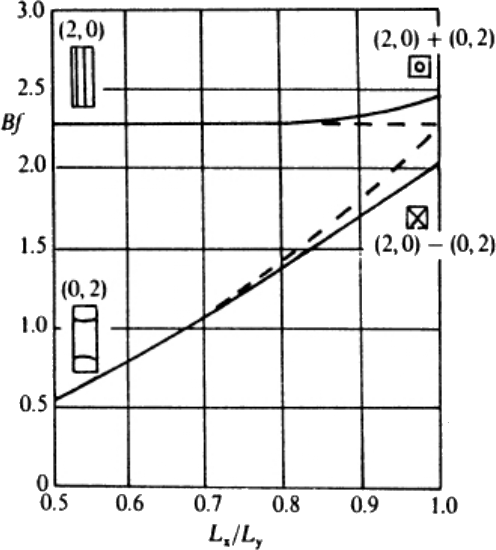
\includegraphics[width=0.5\linewidth]{00_Images/03_chapter/14.png}
    \caption{Frequencies of the vibrational modes as a function of the aspect ratio}
    \label{fig:rect_plate_mode_mixing}
\end{figure}

\section{Bending Waves in Square Plates}

\begin{figure}[!htb]
    \centering
    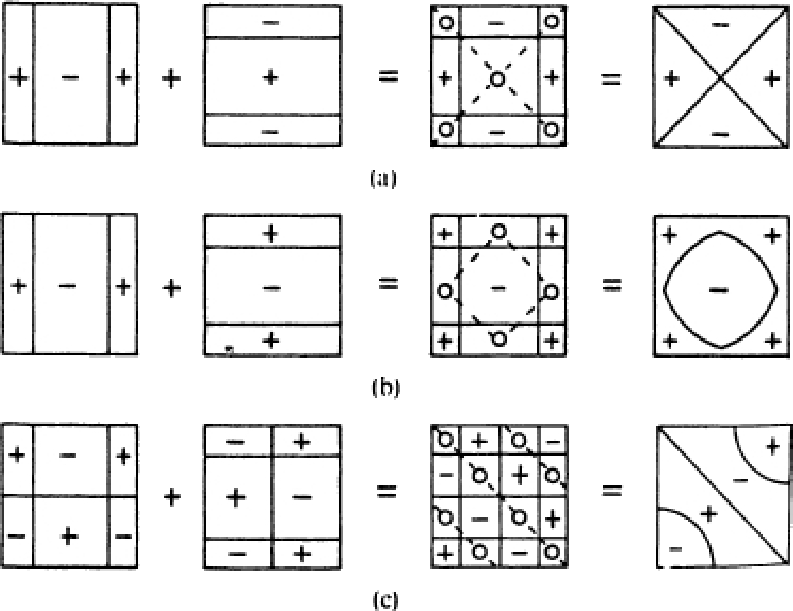
\includegraphics[width=0.7\linewidth]{00_Images/03_chapter/15.png}
    \caption{Graphical construction of the interaction between different modes of a square plate}
    \label{fig:square_plate_modes}
\end{figure}

Square plates (\( L_x = L_y = L \)) are a special case because symmetry forces pairs of rectangular-plate modes \( (m,n) \) and \( (n,m) \) to interact. In membranes this interaction leads to true degeneracy (same frequency). In thin plates, instead, Poisson coupling modifies the stiffness and can split the frequencies of the mixed combinations.

\subsection{Complete Mixing of \texorpdfstring{ \( (2,0) \) }{(2,0)} and \texorpdfstring{ \( (2,0) \) }{(2,0)}: Ring and X Modes}

In a square plate, the two rectangular-plate patterns \( (2,0) \) and \( (0,2) \) are completely mixed. The physically observed shapes are their symmetric and antisymmetric combinations:
\[
(2,0)\pm(0,2)
\]
These are commonly referred to as the ring mode (`` \( + \) '' combination) and the x mode (`` \( - \) '' combination), due to their nodal-line geometry. Unlike the membrane case, the two combinations do not generally have the same eigenfrequency: the relative phase offset between the two component deformations can increase the effective stiffness, producing a frequency split. It reports the following ratio between the two frequencies:
\[
\frac{f_{+}}{f_{-}}
 = 
\sqrt{\frac{1+0.7205\nu}{1-0.7205\nu}}
\]
where \( \nu \) is Poisson's ratio and \( f_{\pm} \) correspond to the \( (2,0)\pm(0,2) \) combinations. For \( \nu = 0.3 \),
\[
\frac{f_{+}}{f_{-}} \approx 1.24
\]

\subsection{Mode Degeneracy for Other Pairs and Excitation Dependence}

The same graphical construction can be applied to other mode pairs, for instance \( (2,1) \) and \( (1,2) \), producing \( (2,1)\pm(1,2) \) and similarly \( (3,1)\pm(1,3) \). A key result reported is that the combinations \( (2,1)\pm(1,2) \) preserve the original modal frequency, i.e. they remain degenerate. As a consequence, which of the two combinations is actually excited depends on where the plate is driven: the driving point selects the modal superposition by projection onto the local modal value. It can be shown that the mode combination does not degenerate (i.e. frequencies split) when
\[
m-n = \pm 2,\pm 4,\pm 6,\dots
\]
which explains why the \( (2,0) \) and \( (0,2) \) pair (difference \( 2 \)) yields distinct ring and x frequencies.

\subsection{Free Edges}

For a square plate with free edges, the first modes and their relative frequencies are conveniently normalized by the lowest-frequency mode \( (1,1) \). The reference frequency is
\[
f_{11} = \frac{h c_L}{L^{2}}\sqrt{\frac{1-\nu}{2}},
\qquad
c_L = \sqrt{\frac{E}{\rho(1-\nu^{2})}}
\]
The first ten modes (relative to \( f_{11} \)) are reported as:
\[
(1,1):1.00,\quad
(2,0)-(0,2):1.52,\quad
(2,0)+(0,2):1.94,\quad
(2,1):2.71,\quad
(1,2):2.71
\]
\[
(2,2):4.81,\quad
(3,0):5.10,\quad
(0,3):5.10,\quad
(3,1)-(1,3):5.30,\quad
(3,1)+(1,3):6.00
\]

\subsection{Clamped Edges}

For clamped edges, the numbering used does not count nodal lines located at the boundaries. The fundamental is the \( (0,0) \) mode, with frequency
\[
f_{00} = 1.654\frac{c_L h}{L^{2}}
\]
The first modes (relative to \( f_{00} \)) are reported as:
\[
(0,0):1.00,\quad
(1,0):2.04,\quad
(0,1):2.04,\quad
(1,1):3.01
\]
\[
(2,0)-(0,2):3.66,\quad
(2,0)+(0,2):3.67,\quad
(2,1):4.58,\quad
(1,2):4.58
\]

Compared with free edges, the transition from the rectangular-plate families to the square-plate mixed patterns is more abrupt with clamped supports. Also remark that ring and x modes are closer in frequency than for free edges and that some mode frequencies (notably \( (1,1) \)) are strongly shifted upward with clamping.

\section{Rectangular Wood Plates}

Plates used in musical instruments are rarely isotropic. Wood is strongly anisotropic and is commonly modeled as an orthotropic elastic medium, with three privileged material axes: longitudinal \( L \) (along the fibers), radial \( R \) (across growth rings) and tangential \( T \) (tangent to growth rings). This directional elasticity has immediate consequences on mode shapes, modal degeneracies and eigenfrequency trends with geometry.

\subsection{Orthotropic Parameters and Quarter-Cut Plates}

To characterize a generic wood plate one needs three Young's moduli \( (E_L,E_R,E_T) \) and either six Poisson ratios \( \nu_{ij} \) (two for each pair of directions) or, equivalently, three Poisson ratios together with three shear moduli. The reciprocity relations
\[
\frac{\nu_{ij}}{E_i} = \frac{\nu_{ji}}{E_j},
\qquad i,j\in\{L,R,T\}
\]
reduce the number of independent coefficients. In instrument, plates are often quarter-cut, i.e. cut along two radii so that the \( L \) and \( R \) axes lie in the plate plane while the \( T \) axis is aligned with thickness. In this common configuration, four elastic constants are sufficient to capture the dominant vibrational behavior:
\[
E_L,\qquad E_R,\qquad G \ (\text{in-plane shear}),\qquad \nu_{LR}\ (\text{or equivalently } \nu_{RL})
\]

\subsection{Consequences for Mode Shapes}

%\begin{figure}[!htb]
%    \centering
%    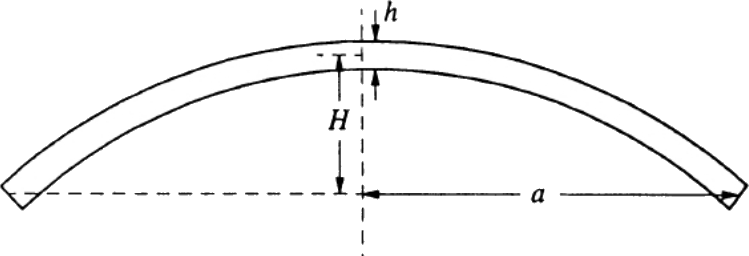
\includegraphics[width=0.9\linewidth]{00_Images/03_chapter/17.png}
%    \caption{Example mode shapes of a violin back plate}
%    \label{fig:violin_back_modes}
%\end{figure}

A key qualitative fact is that in wood typically \( E_L>E_R \). As a result, the mode families and degeneracies that are observed in a square isotropic plate do not generally occur in a square wood plate: the stiffness contrast along \( L \) and \( R \) breaks the symmetry between the two in-plane directions. To recover mode patterns analogous to the isotropic-square case one must choose a non-square aspect ratio satisfying
\[
\frac{L_x}{L_y} = \left(\frac{E_L}{E_R}\right)^{1/4}
\]
For Sitka spruce this gives approximately
\[
\frac{L_x}{L_y} \simeq 1.9
\]
In violin making, modes with patterns similar to the so-called x-mode and ring-mode are indeed observed on top and back plates and are used to tune plates before assembly. As an example reported for a violin back plate, mode shapes labeled 2 and 5 resemble x- and ring-like patterns (with indicative frequencies around 165 Hz and 350 Hz, respectively), alongside a lower mode around 85 Hz. 

\subsection{Simply Supported Orthotropic Plate: Modal Frequency Formula}

The frequency formulas derived for isotropic plates can be adapted to wood by replacing \( E \) with the appropriate directional modulus and replacing the isotropic Poisson combination \( \nu^{2} \) with the orthotropic product \( \nu_{xy}\nu_{yx} \). For a rectangular wood plate with simply supported edges, the \( (m,n) \) -th modal frequency is given as
\[
f_{mn}
 = 
0.453h
\left[
c_x\left(\frac{m+1}{L_x}\right)^{2}
+
c_y\left(\frac{n+1}{L_y}\right)^{2}
\right],
\qquad m,n = 0,1,2,\dots
\]
where the directional wave-speed-like parameters are
\[
c_x = \sqrt{\frac{E_x}{\rho\left(1-\nu_{xy}\nu_{yx}\right)}},
\qquad
c_y = \sqrt{\frac{E_y}{\rho\left(1-\nu_{yx}\nu_{xy}\right)}}
\]
In a quarter-cut plate one typically identifies \( x = L \) and \( y = R \), so that \( E_x = E_L \), \( E_y = E_R \) and the anisotropy enters explicitly through \( c_x\neq c_y \).

\section{Vibration in Shells}

\begin{figure}[!htb]
    \centering
    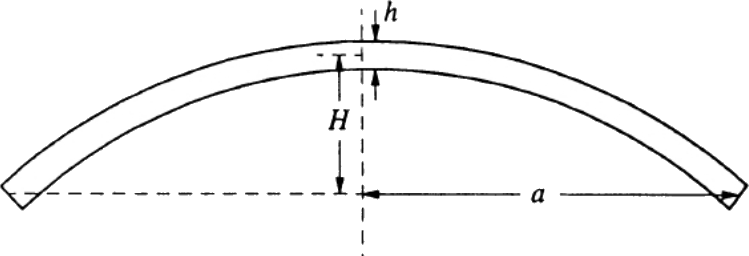
\includegraphics[width=0.9\linewidth]{00_Images/03_chapter/17.png}
    \caption{Effect of curvature on shell vibration and arching}
    \label{fig:shell_arching}
\end{figure}

Shells are thin curved surfaces. Compared with flat plates, curvature (arching) increases stiffness and has two immediate consequences in musical-acoustics structures:

\begin{enumerate}
    \item Static benefit arched parts can bear higher loads with less reinforcement. For example, the arched violin top plate can withstand string tension with only minor bracing (bass bar), while the flat guitar top plate typically requires substantial bracing to avoid yielding under the same type of load.
    \item Dynamic benefit: the vibrational response is modified: eigenfrequencies and mode families change because curvature couples bending and in-plane deformation.
\end{enumerate}

\subsection{Extensional vs Nonextensional Modes and Thickness Dependence}

Two limiting families of shell modes can be distinguished.

\begin{itemize}
    \item Extensional modes: vibrations that change the length of (at least) one line drawn on the shell surface. Their frequency is essentially independent of the thickness \( h \).
    \item Nonextensional modes: vibrations that do not change the length of any line on the shell (in the idealized sense). Their frequency is proportional to \( h \).
\end{itemize}

In practical shell geometries the separation is not always clean: modes may be partly extensional and partly nonextensional. A compact way to express this mixed dependence is
\[
f_{mn} = \left(A_{mn}+B_{mn}h^{2}\right)^{1/2}
\]
showing that thickness enters progressively (through the \( B_{mn}h^{2} \) term) rather than as an all-or-nothing classification.

\subsection{Spherical Shells: Lowest Axisymmetric Mode and Arching Effects}

Consider a spherical-cap shell of radius \( a \), thickness \( h \) and rise (depth) \( H \). When \( H = 0 \), the structure reduces to a flat circular plate and the lowest mode satisfies
\[
ka = \mu_0
\]
where \( \mu_0 \) depends on the boundary condition (as in the circular-plate formulas). When \( H\neq 0 \), curvature shifts the lowest mode so that approximately
\[
ka  \simeq \mu,
\qquad
\mu \approx
\begin{cases}
3, & \text{free edges or clamped edges with } H \text{ comparable to } h\\
6, & \text{clamped edges with } H \gg h
\end{cases}
\]

A more detailed prediction for the frequency of the lowest axisymmetric mode (displacement depending on \( r \) but not on \( \varphi \)) is given in normalized form as
\[
\frac{\omega}{\omega_0}
 = 
\left[
\frac{1}{1-\nu^{2}}\left(\frac{\mu}{\mu_0}\right)^{4}
+
\frac{48}{\mu_0^{4}}\left(\frac{H}{h}\right)^{2}
\right]^{1/2}
\]
where \( \omega_0 \) is the lowest-mode frequency of the flat circular plate with the same boundary conditions. This expression makes the role of arching explicit:

\begin{itemize}
    \item for a violin top plate, where the arching is typically a bit larger than the thickness, one finds approximately \( \omega  \simeq 2\omega_0 \);
    \item when \( H \ll h \), curvature is negligible and \( \omega \simeq \omega_0 \);
    \item for larger \( H/h \), it reports the asymptotic linear scalings
    \[
    \frac{\omega}{\omega_0} = 0.68\frac{H}{h}\quad \text{(clamped edges)},
    \qquad
    \frac{\omega}{\omega_0} = 0.84\frac{H}{h}\quad \text{(free edges)}
    \]
\end{itemize}

Finally, for a shell that is both thin and shallow (\( H/h\ge 20 \) and \( H/a<0.25 \)), the lowest frequency can be approximated directly by material and geometry
\[
\omega \simeq 2\left(\frac{E}{\rho}\right)^{1/2}\frac{H}{a^{2}}
\]

\subsection{Cylindrical Shells: Two Musical-Acoustics Applications}

Cylindrical shells appear in two relevant contexts. 

\begin{enumerate}
    \item Drum shells: the shell acts as a support structure for a light membrane. Two shell modes are especially important:
    \begin{itemize}
        \item a lowest extensional (breathing) mode, involving radial motion of the shell wall;
        \item a nonextensional mode involving ovalization (the cross-section becomes elliptical).
    \end{itemize}
    These become particularly relevant when the shell itself is excited by sticks.
    \item Orchestral chimes (tubular bells): tubes behave similarly to bars but with shape dependent corrections. It reports that bending-mode frequencies decrease when the cylinder is not perfectly rectilinear.
\end{enumerate}

\section{Driving-Point Impedance}

For continuous structures, the response to excitation depends not only on frequency but also on where the system is driven and where the motion is observed. A compact quantity that summarizes this dependence is the mechanical impedance, defined as the ratio between applied force and resulting velocity. 

\subsection{Definition and Measurement}

\begin{figure}[!htb]
    \centering
    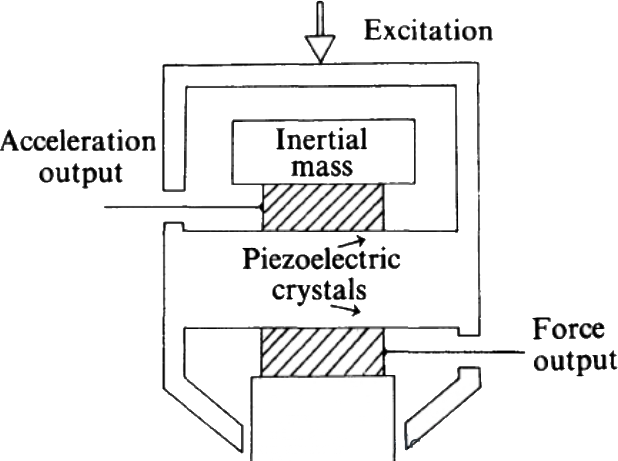
\includegraphics[width=0.7\linewidth]{00_Images/03_chapter/18.png}
    \caption{Impedance-head measurement of driving-point impedance}
    \label{fig:impedance_head}
\end{figure}

The (transfer) mechanical impedance between an excitation point \( \vv{r_F} \) and an observation point \( \vv{r_v} \) is
\[
Z(\omega;\vv{r_F},\vv{r_v}) = \frac{F(\omega;\vv{r_F})}{v(\omega;\vv{r_v})}
\]
In general, \( Z \) varies with the locations of the input and output points. A particularly important case is the driving-point (or input) impedance, obtained when force and velocity are measured at the same point:
\[
Z_{\mathrm{in}}(\omega;\vv{r_0}) = \frac{F(\omega;\vv{r_0})}{v(\omega;\vv{r_0})}
\]
Its reciprocal,
\[
Y_{\mathrm{in}}(\omega;\vv{r_0}) = \frac{1}{Z_{\mathrm{in}}(\omega;\vv{r_0})} = \frac{v(\omega;\vv{r_0})}{F(\omega;\vv{r_0})}
\]
is the driving-point admittance (mobility). 

\paragraph{Impedance head} A practical way to measure \( Z_{\mathrm{in}} \) is an impedance head, which combines a force sensor and an accelerometer (or velocity sensor) in one device. The head is attached to an electromagnetic shaker, which can generate pseudo-random sequences or swept-sine excitation. A crucial experimental detail is that the head has its own inertial mass \( m \), which loads the structure and therefore modifies the measured impedance if the attachment point is light.

\subsection{Infinite vs Finite Structures}

For an infinite structure there are no reflections, so the driving-point impedance is closely related to the characteristic wave impedance of the propagating wave.

\paragraph{Examples (infinite structures)} It lists the following relevant results. 

\begin{itemize}
    \item Longitudinal wave in an infinite bar:
    \[
    Z = \mu c_L
    \]
    where \( \mu \) is the mass per unit length and \( c_L \) is the longitudinal wave speed.
    \item Bending waves in an infinite bar:
    \[
    Z(f) = \mu v(f)\frac{1+j}{2}
    \]
    so the magnitude increases as \( \sqrt{f} \) (because the bending-wave phase velocity \( v(f) \propto \sqrt{f} \)).
    \item Infinite thin plate: the driving-point impedance is constant with frequency (a hallmark of 2D bending-wave spreading) and it can be written in terms of the bending stiffness
    \[
    D = \frac{E h^{3}}{12(1-\nu^{2})}
    \]
    as
    \[
    Z = 8\sqrt{\rho_sD}
    \qquad
    \left(\rho_s = \sigma = \rho h\ \text{mass per unit area}\right)
    \]
\end{itemize}

For finite structures, reflections from boundaries produce standing-wave resonances. As a result, the driving-point impedance (or admittance) shows sharp peaks and dips associated with the eigenmodes and the detailed curve depends strongly on the measurement point (nodal/antinodal location). This is illustrated by:

\begin{itemize}
    \item the driving-point impedance of a finite bar measured at an endpoint for different damping factors;
    \item the driving-point admittance of a finite plate measured at two different surface points, yielding visibly different resonance patterns.
\end{itemize}

\paragraph{Effect of damping} The damping factor is expressed as
\[
\frac{2\alpha}{\omega_0} = \frac{1}{Q}
\]
Increasing damping reduces the sharpness of resonance features: peaks are broader and lower and the impedance curve becomes smoother as the modal overlap increases.

\begin{figure}[!htb]
    \centering
    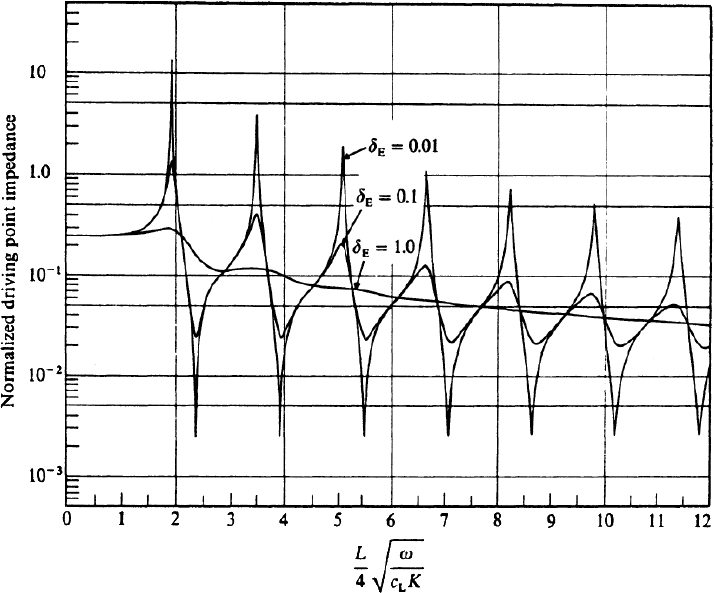
\includegraphics[width=0.75\linewidth]{00_Images/03_chapter/19.png}
    \caption{Driving-point impedance/admittance in finite structures}
    \label{fig:Driving_point_admittance}
\end{figure}

\section{Coupling Between Vibrating Systems}

When two vibrating structures can exchange vibrational energy, the behavior of the coupled assembly can differ significantly from the behavior of each structure in isolation. In musical instruments this situation is ubiquitous: a string drives a bridge, the bridge drives a soundboard, and the soundboard interacts with the enclosed air. The key point is that coupling is not just an ``energy leak'': if the coupled structure has its own resonances, it can shift or split the resonances of the driven structure. 

\subsection{Springlike and Masslike Terminations Around a Resonance}

As already encountered the special case of a string ended by a termination that is purely masslike or purely springlike, which systematically raises or lowers the resonance frequencies. The more general (and more realistic) case is when the termination itself is resonant (e.g. a bridge with its own modes). Then the termination impedance is frequency dependent and changes qualitative character across its resonance. In particular, denoting the termination impedance by \( Z_b(\omega) \), its imaginary part determines whether the termination behaves as a spring or a mass:
\[
\Im\{Z_b(\omega)\}<0 \quad\Rightarrow\quad \text{springlike behavior},
\qquad
\Im\{Z_b(\omega)\}>0 \quad\Rightarrow\quad \text{masslike behavior}
\]
For a bridge resonance close to a string resonance:

\begin{itemize}
    \item below the bridge resonance, the bridge appears springlike;
    \item above the bridge resonance, the bridge appears masslike.
\end{itemize}

As a consequence, the resonances of the string are pushed away from the bridge resonance and can be split into two nearby peaks: the coupled system reorganizes its modal structure.

\subsection{Weak vs Strong Coupling}

Coupling does not always produce a dramatic modification of the spectrum. Two regimes can be distinguished.

\paragraph{Weak coupling} The eigenfrequencies of the structure where the vibration is generated are essentially unaffected by the other structure. In this case, a sequential (one-way) approach is acceptable for vibroacoustic characterization:

\begin{itemize}
    \item compute the vibrational response of the first structure neglecting interaction;
    \item use that response as the excitation (initial condition / boundary input) for the second structure.
\end{itemize}

\paragraph{Strong coupling} The interaction modifies the eigenfrequencies of both structures. Then a sequential approach fails: one must solve the vibroacoustic response of the coupled system simultaneously (one set of equations with mutual interaction). The transition between weak and strong coupling depends on the properties of the two structures and, crucially, on frequency.

\section{Coupling Criteria}

The weak/strong coupling distinction becomes quantitative once one introduces dimensionless parameters comparing the characteristic impedances (and stored energy) of the interacting subsystems. This section summarizes two standard criteria from musical acoustics: coupling between a plate and the surrounding air, and coupling between a string and a soundboard.

\subsection{Coupling Between a Plate and Air}

A relevant example is a vibrating plate surrounded by air. In this case the weak/strong coupling regime is governed by the dimensionless parameter 
\[
\beta_c = \frac{\rho_0 c_0}{\rho_s h_s\,\omega_c}
\]
where

\begin{itemize}
    \item \( h_s \) is the plate thickness,
    \item \( \rho_s \) is the density of the structure (plate material),
    \item \( \rho_0 \) is the density of the fluid (air),
    \item \( c_0 \) is the sound speed in the fluid,
    \item \( \omega_c \) is the critical angular frequency of the plate, i.e. the frequency above which the plate can radiate sound efficiently.
\end{itemize}

The criterion reported in the slides is: 
\[
\beta_c  \ll 1 \quad \Rightarrow \quad \text{weak coupling},
\qquad
\beta_c \gtrsim 1 \quad \Rightarrow \quad \text{strong coupling}
\]
\paragraph{Remark} In this plate-air case, the slides explicitly note that the classification as weak/strong coupling does not depend on frequency (the relevant frequency scale is already embedded in \( \omega_c \)). 

\subsection{String Coupled to a Soundboard: Weak and Strong Coupling}

The coupling between a string and a soundboard can also be weak or strong. The slides express the regime in terms of the dimensionless ratio \( m/(n^2M) \), where:

\begin{itemize}
    \item \( m \) is the mass of the string,
    \item \( M \) is the effective mass of the soundboard (for the relevant resonance),
    \item \( n \) is the string mode number,
    \item \( Q_B \) is the merit factor (quality factor) of the soundboard resonance.
\end{itemize}

\begin{figure}[!htb]
    \centering
    \subfloat[Strong]{%
        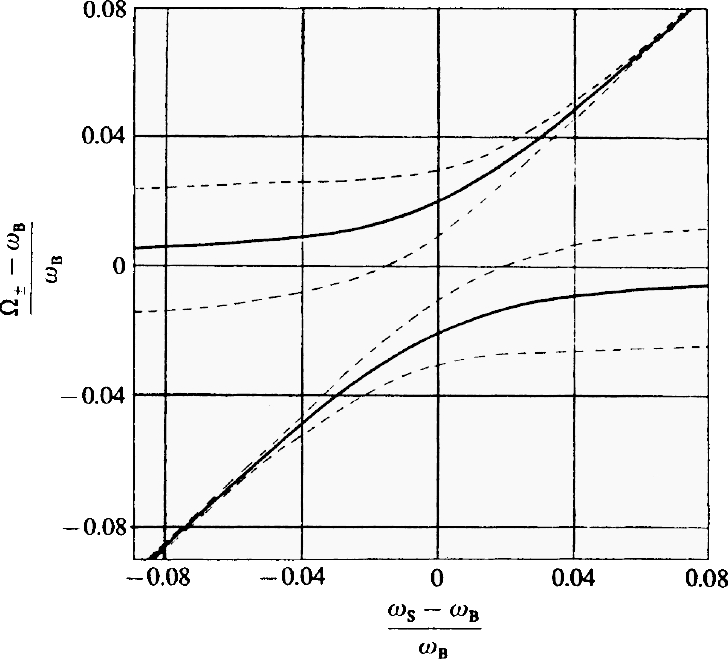
\includegraphics[height=0.25\textheight]{00_Images/03_chapter/21.png}%
    }\hfill
    \subfloat[Weak]{%
        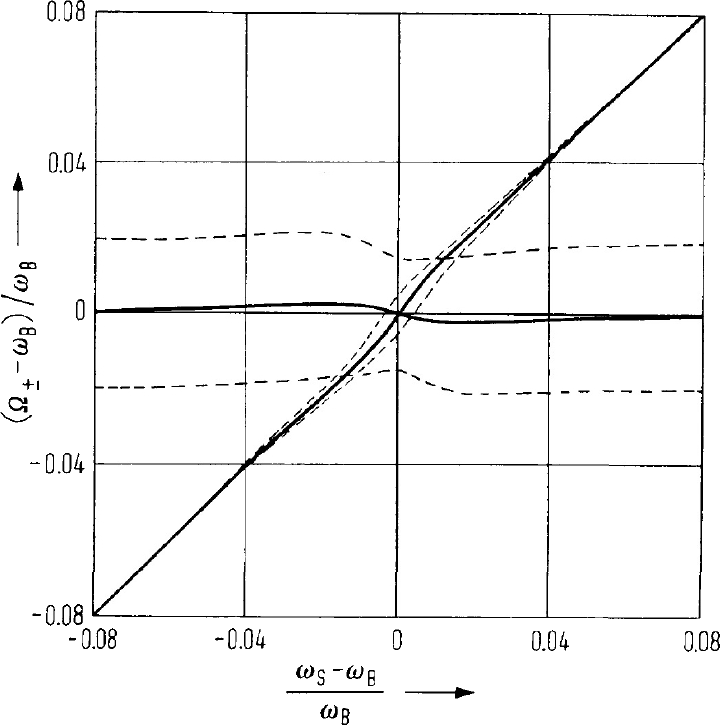
\includegraphics[height=0.25\textheight]{00_Images/03_chapter/22.png}%
    }
    \caption{Weak vs strong coupling between a string mode and a soundboard resonance}
    \label{fig:string_soundboard_coupling}
\end{figure}

\paragraph{Weak coupling} Weak coupling occurs when
\[
\frac{m}{n^{2}M}<\frac{\pi^{2}}{4Q_B^{2}}
\]
In this regime, if a string mode and a soundboard mode originally coincide in frequency, the coupling does not significantly alter their normal-mode frequencies. What changes instead is the damping: energy leakage into the soundboard modifies decay rates, while the resonance locations remain essentially those of the uncoupled subsystems.

\paragraph{Strong coupling and mode splitting} Strong coupling occurs when
\[
\frac{m}{n^{2}M}>\frac{\pi^{2}}{4Q_B^{2}}
\]
If the two uncoupled resonances coincide at \( \omega_0 \) (i.e. \( \omega_n = \omega_B = \omega_0 \)), the slides state that the normal modes are split symmetrically about \( \omega_0 \), and their damping factor becomes \( 2Q_B \).

\paragraph{Graphical interpretation} The plotted curves in the slides show that the normalized separation of the two coupled frequencies increases with \( m/(n^2M) \), and that the amount of splitting depends on \( Q_B \): higher- \( Q_B \) boards (sharper resonances) exhibit a more pronounced separation for the same mass ratio. A second plot summarizes the overall behavior by showing avoided crossing and symmetric splitting in the strong-coupling case and nearly unchanged resonance lines (but altered damping) in the weak-coupling case.

\section{Two Strings Coupled by a Bridge}

This configuration is relevant in string instruments whenever two strings are tuned at very close frequencies (a typical example is unison strings in the piano). We consider two strings that are identical in length \( L \), density \( \rho \), cross-sectional area \( S \), and linear density \( \mu = \rho S \), but differ in their tensions \( T_1 \) and \( T_2 \). Their transverse displacements are denoted \( y_1(x,t) \) and \( y_2(x,t) \).

\subsection{Governing Equations and Bridge Boundary Conditions}

\begin{figure}[!htb]
    \centering
    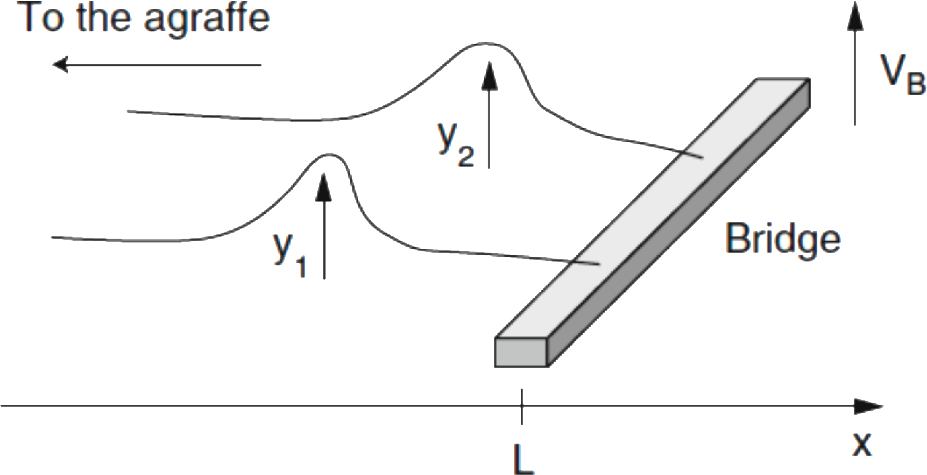
\includegraphics[width=0.8\linewidth]{00_Images/03_chapter/23.png}
    \caption{Two strings coupled by a bridge: schematic model}
    \label{fig:two_strings_bridge}
\end{figure}

Each string satisfies the (lossless) wave equation
\[
\left\{
\begin{aligned}
\rho S\,\frac{\partial^2 y_1}{\partial t^2}-T_1\,\frac{\partial^2 y_1}{\partial x^2}& = 0\\
\rho S\,\frac{\partial^2 y_2}{\partial t^2}-T_2\,\frac{\partial^2 y_2}{\partial x^2}& = 0
\end{aligned}
\right.
\]
The ends far from the bridge are fixed. At the bridge (\( x = L \)) the two strings share the same displacement,
\[
y_1(L,t) = y_2(L,t) = q_B(t)
\]
where \( q_B(t) \) is the bridge displacement. The bridge is characterized (in the frequency range of interest) by a mechanical impedance \( Z_B \), so that
\[
F_B(\omega) = Z_B(\omega)\,V_B(\omega),
\qquad
V_B = j\omega q_B
\]
The total force exerted by the two strings on the bridge is the sum of the end forces
\[
F_B = F_1+F_2
 = -T_1\left.\frac{\partial y_1}{\partial x}\right|_{x = L}
   -T_2\left.\frac{\partial y_2}{\partial x}\right|_{x = L}
\]

\subsection{Reduced Modal Model Near Unison}

The displacement of each string can be expanded onto its eigenmodes,
\[
y_1(x,t) = \sum_{n = 1}^{N}\phi_{1n}(x)\,q_{1n}(t),
\qquad
y_2(x,t) = \sum_{n = 1}^{N}\phi_{2n}(x)\,q_{2n}(t)
\]
For bridges with reduced mobility, the mode shapes remain close to the fixed-end shapes,
\[
\phi_{in}(x) \simeq \sin(k_n x),\qquad i = 1,2
\]
and the deviations from ideal fixed-end behavior are concentrated in the generalized coordinates \( q_{in}(t) \). Restricting attention to the fundamental modes gives
\[
y_1(x,t) \simeq \phi_1(x)\,q_1(t),\qquad
y_2(x,t) \simeq \phi_2(x)\,q_2(t)
\]
and we may write the two uncoupled oscillators schematically as
\[
\left\{
\begin{aligned}
\ddot{q}_1+\omega_1^2 q_1 & = g_1(q_i)\\
\ddot{q}_2+\omega_2^2 q_2 & = g_2(q_i)
\end{aligned}
\right.
\]
where the coupling effects are included in the perturbation terms \( g_i \). We seek complex-frequency solutions \( q_i(t) \propto e^{j\beta t} \) (with \( \beta \) complex to include attenuation), which leads to
\[
(\omega_0^2-\beta^2)\psi_1 = \gamma_1(\psi_i),
\qquad
(\omega_0^2-\beta^2)\psi_2 = \gamma_2(\psi_i)
\]
where \( \psi_i \) are complex amplitudes.
If detuning is small, the bridge impedance can be approximated as \( Z_B(\omega) \simeq Z_B(\omega_0) \), and it is convenient to work with the bridge admittance \( Y_B = 1/Z_B \). Using the end impedance of a string,
\[
Z = jZ_c\cot(kL)
\]
and expanding \( \cot(\cdot) \) around the fundamental, one obtains (near \( \omega_0 \)) a local relation between the end force and the bridge velocity. Specializing to the two strings yields the coupled system
\[
\left\{
\begin{aligned}
(\omega_1^2-\beta^2)F_1 & = -\frac{2T_1}{L}\,j\beta\,Y_B\,(F_1+F_2)\\
(\omega_2^2-\beta^2)F_2 & = -\frac{2T_2}{L}\,j\beta\,Y_B\,(F_1+F_2)
\end{aligned}
\right.
\]

\subsection{Detuning Parameter and Eigenvalues}

Let the two strings be slightly detuned by writing
\[
\omega_1 = \omega_0,
\qquad
\omega_2 = \omega_0(1+2\epsilon)
\]
which corresponds (to first order) to \( T_2 = T_1(1+4\epsilon) \).
With this parametrization, the coupled system can be reduced to
\[
\left\{
\begin{aligned}
j(\beta-\omega_0)F_1 & = j\zeta(F_1+F_2)\\
j(\beta-\omega_0)F_2 & = j\zeta(F_1+F_2)+2j\epsilon\omega_0 F_2
\end{aligned}
\right.
\]
where \( \zeta \) is a normalized coupling coefficient proportional to \( Y_B \).
Writing \( \beta = \omega_0+\alpha \) and introducing the dimensionless quantities
\[
a = \frac{\alpha}{\omega_0},\qquad \chi = \frac{\zeta}{\omega_0}
\]
one obtains the eigenproblem
\[
ja
\begin{bmatrix}
F_1\\F_2
\end{bmatrix}
 = 
j
\begin{bmatrix}
\chi & \chi\\
\chi & \chi+2\epsilon
\end{bmatrix}
\begin{bmatrix}
F_1\\F_2
\end{bmatrix}
\]
The eigenvalues \( a_\pm \) follow from
\[
a^{2}-2a(\chi+\epsilon)+2\epsilon\chi = 0
\qquad\Longrightarrow\qquad
a_\pm = \chi+\epsilon\pm\sqrt{\epsilon^{2}+\chi^{2}}
\]
The real part of \( a_\pm \) determines the eigenfrequency shift, while the imaginary part determines the damping factor.

\subsection{Reactive, Resistive, and Complex Bridge Admittance}

Different behaviors occur depending on the nature of the bridge admittance \( Y_B \), i.e. of \( \chi \).

\paragraph{Purely Reactive Admittance} If \( Y_B \) is purely reactive, then \( \chi = \xi\in\mathbb{R} \). The eigenfrequencies (real part of \( a_\pm \)) approach the uncoupled values when \( |\epsilon| \) is large, while in the unison limit \( \epsilon\to 0 \) the coupling becomes dominant and the two eigenfrequencies move apart (avoided crossing / splitting). Since \( \chi \) is real, no additional damping is introduced by the bridge in this idealized reactive case.

\paragraph{Purely Resistive Admittance} If \( Y_B \) is purely resistive, then \( \chi = j\eta \) with \( \eta>0 \). Two regimes arise:

\begin{itemize}
    \item If \( \epsilon>\eta \), then
    \[
    a_\pm = \epsilon+j\eta\pm\sqrt{\epsilon^{2}-\eta^{2}}
    \]
    so the eigenfrequency shifts (real parts) follow two hyperbola-like branches, while the damping (imaginary part) remains constant and equal to \( \eta \).
    \item If \( \eta>\epsilon \), the real part collapses to the line segment
    \[
    \Re\{a_\pm\} = \epsilon
    \]
    while the imaginary parts trace a circle in the complex plane (center at \( j\eta \), radius \( \eta \)), corresponding to a redistribution of damping between the two coupled modes.
\end{itemize}

\paragraph{Complex Admittance and Damping Redistribution} If \( Y_B \) is complex, \( \chi = \xi+j\eta \), an intermediate situation occurs. The coupling modifies eigenfrequencies and damping significantly only for sufficiently small detuning \( \epsilon \). A striking result in the unison limit (\( \epsilon = 0 \)) is that one of the two eigenmodes can become essentially undamped while the other becomes strongly damped: it is as if the bridge dissipation is pumped by one mode out of the two, leaving the other mode to survive for a much longer time.

\begin{figure}[!htb]
    \centering
    \subfloat[Real Part]{
        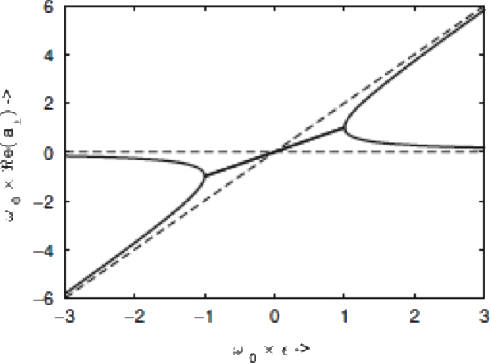
\includegraphics[height=0.2\textheight]{00_Images/03_chapter/24.png}
    }
    \hfill
    \subfloat[Immaginary Part]{
        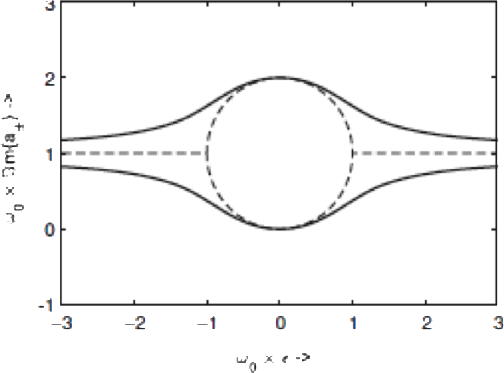
\includegraphics[height=0.2\textheight]{00_Images/03_chapter/25.png}
    }
    \caption{Bridge admittance}
    \label{fig:bridge_admittance_cases}
\end{figure}

\subsection{Time-Domain Interpretation}

\begin{figure}[!htb]
    \centering
    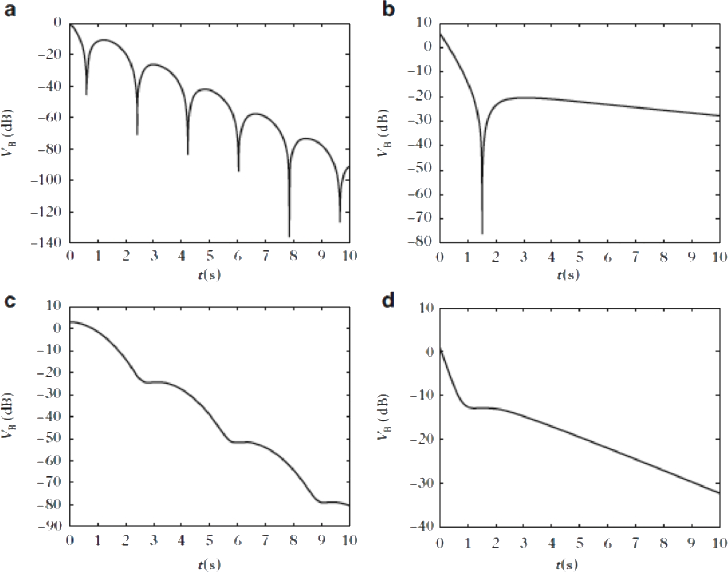
\includegraphics[width=0.85\linewidth]{00_Images/03_chapter/26.png}
    \caption{Time-domain responses for different coupling regimes}
    \label{fig:coupling_time_domain}
\end{figure}

Once \( F_1(t) \) and \( F_2(t) \) are reconstructed from the modal decay rates associated with \( a_{\pm} \), the bridge velocity is obtained as
\[
V_B = Y_B(F_1+F_2)
\]
The corresponding time responses can have very different envelopes. With mainly resistive coupling (large \( \eta \)) the decay is dominated by dissipation, while mainly reactive coupling (large \( \xi \)) tends to emphasize beating. For a genuinely complex admittance, it is common to observe an uneven redistribution of damping: one component decays quickly, leaving a slowly decaying residual motion linked to the weakly damped coupled mode.

\section{Nonlinear Effects in Shells and Plates}

Up to now, the governing equations have been treated as linear, so that mode shapes and eigenfrequencies are independent of vibration amplitude. In real plates and shells this assumption can break down when the deflection becomes large compared to the thickness (or to the shell curvature depth). In that case, geometric nonlinearities introduce an amplitude-dependent stiffness, and therefore the modal frequencies are no longer constant.

\begin{figure}[!htb]
    \centering
    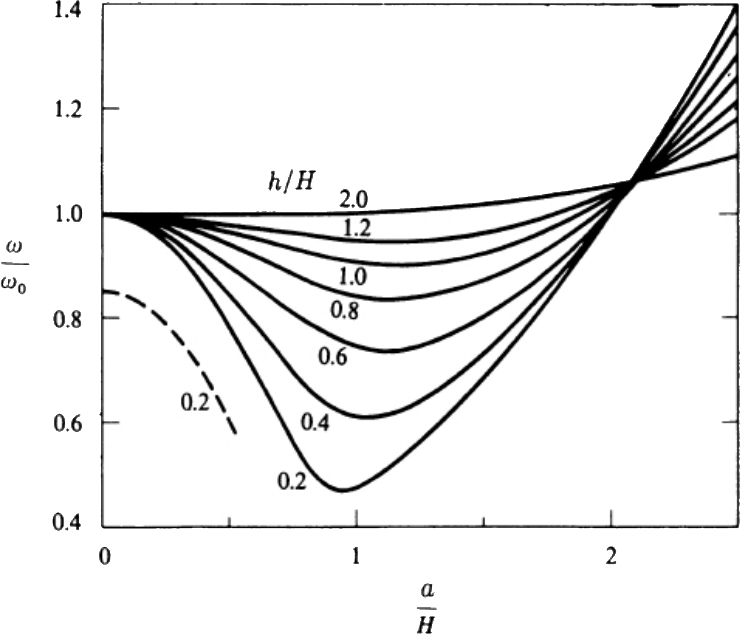
\includegraphics[width=0.6\linewidth]{00_Images/03_chapter/27.png}
    \caption{Typical nonlinear frequency shift in plates/shells with increasing amplitude}
    \label{fig:nonlinear_shift}
\end{figure}

\subsection{Amplitude-Dependent Frequency in a Circular Plate}

A simple (and very useful) rule of thumb is given for a flat circular plate of thickness \( h \), vibrating with displacement amplitude \( a \). The oscillation frequency increases with amplitude according to the approximation
\[
\omega  \approx \omega_0\left[1 + 0.16\left(\frac{a}{h}\right)^2\right]
\]
where \( \omega_0 \) is the small-amplitude (infinitesimal) angular frequency. This effect is especially relevant in instruments such as gongs, where vibration amplitudes can be large enough that audible pitch glide occurs during the decay.

\subsection{Nonlinear Behavior in Shells}

For shells the picture becomes more complex because the curvature couples bending and in-plane stretching. The slides summarize the behavior in terms of the frequency ratio \( \omega/\omega_0 \) as a function of the normalized amplitude \( a/H \), where \( H \) is the cap height, and for different values of the thickness ratio \( h/H \).

\paragraph{Thin shells: tension-dominated nonlinearity} If the shell is very thin, \( h/H  \ll 1 \), nonlinear tension effects dominate the response. As the vibration amplitude increases towards the shell depth (\( a \to H \)), the mode frequency can drop to about half of its small-amplitude value. A further increase in amplitude causes the frequency to rise again. 

\paragraph{Thicker shells: bending-dominated response} As the ratio \( h/H \) increases, bending stiffness becomes more important and the nonlinear effect weakens. The ratio \( \omega/\omega_0 \) stays closer to unity, and the frequency shift with amplitude becomes less evident.

